%%%%%%%%%%%%%%%%%%%%%%%%%%%%%%%%%%%%%%%
% Wenneker Resume/CV
% LaTeX Template
% Version 1.1 (19/6/2016)
%
% This template has been downloaded from:
% http://www.LaTeXTemplates.com
%
% Original author:
% Frits Wenneker (http://www.howtotex.com) with extensive modifications by 
% Vel (vel@LaTeXTemplates.com)
%
% License:
% CC BY-NC-SA 3.0 (http://creativecommons.org/licenses/by-nc-sa/3.0/
%
%%%%%%%%%%%%%%%%%%%%%%%%%%%%%%%%%%%%%%

%----------------------------------------------------------------------------------------
%	PACKAGES AND OTHER DOCUMENT CONFIGURATIONS
%----------------------------------------------------------------------------------------

\documentclass[a4paper,12pt]{article} % Font and paper size, changed from memoir to article

%%%%%%%%%%%%%%%%%%%%%%%%%%%%%%%%%%%%%%%%%
% Wenneker Resume/CV
% Structure Specification File
% Version 1.1 (19/6/2016)
%
% This file has been downloaded from:
% http://www.LaTeXTemplates.com
%
% Original author:
% Frits Wenneker (http://www.howtotex.com) with extensive modifications by 
% Vel (vel@latextemplates.com)
%
% License:
% CC BY-NC-SA 3.0 (http://creativecommons.org/licenses/by-nc-sa/3.0/)
%
%%%%%%%%%%%%%%%%%%%%%%%%%%%%%%%%%%%%%%%%%

%----------------------------------------------------------------------------------------
%	PACKAGES AND OTHER DOCUMENT CONFIGURATIONS
%----------------------------------------------------------------------------------------

\usepackage{XCharter} % Use the Bitstream Charter font
\usepackage[utf8]{inputenc} % RequiRoyalBlue for inputting international characters
\usepackage[T1]{fontenc} % Output font encoding for international characters

\usepackage[top=1cm,left=.1cm,right=1cm,bottom=1cm]{geometry} % Modify margins

\usepackage{graphicx} % RequiRoyalBlue for figures

\usepackage{flowfram} % RequiRoyalBlue for the multi-column layout

\usepackage{url} % URLs

\usepackage[usenames,dvipsnames]{xcolor} % RequiRoyalBlue for custom colours

\usepackage{tikz} % RequiRoyalBlue for the horizontal rule

\usepackage{enumitem} % RequiRoyalBlue for modifying lists
\setlist{noitemsep,nolistsep} % Remove spacing within and around lists

\setlength{\columnsep}{\baselineskip} % Set the spacing between columns

% Define the left frame (sidebar)
\newflowframe{0.25\textwidth}{\textheight}{0pt}{0pt}[left]
\newlength{\LeftMainSep}
\setlength{\LeftMainSep}{0.25\textwidth}
\addtolength{\LeftMainSep}{1\columnsep}
 
% Small static frame for the vertical line
\newstaticframe{1.5pt}{\textheight}{\LeftMainSep}{0pt}
 
% Content of the static frame with the vertical line
\begin{staticcontents}{1}
\hfill
\tikz{\draw[loosely dotted,color=RoyalBlue,line width=1.5pt,yshift=0](0,0) -- (0,\textheight);}
\hfill\mbox{}
\end{staticcontents}
 
% Define the right frame (main body)
\addtolength{\LeftMainSep}{1.5pt}
\addtolength{\LeftMainSep}{1\columnsep}
\newflowframe{0.7\textwidth}{\textheight}{\LeftMainSep}{0pt}[main01]

\pagestyle{empty} % Disable all page numbering

\setlength{\parindent}{0pt} % Stop paragraph indentation

%----------------------------------------------------------------------------------------
%	NEW COMMANDS
%----------------------------------------------------------------------------------------

\newcommand{\userinformation}[1]{\renewcommand{\userinformation}{#1}} % Define a new command for the CV user's information that goes into the left column

\newcommand{\cvheading}[1]{{\Huge\bfseries\color{RoyalBlue} #1} \par\vspace{.6\baselineskip}} % New command for the CV heading
\newcommand{\cvsubheading}[1]{{\Large\bfseries #1} \bigbreak} % New command for the CV subheading

\newcommand{\Sep}{\vspace{1em}} % New command for the spacing between headings
\newcommand{\SmallSep}{\vspace{0.5em}} % New command for the spacing within headings

\newcommand{\aboutme}[2]{ % New command for the about me section
\textbf{\color{RoyalBlue} #1}~~#2\par\Sep
}
	
\newcommand{\CVSection}[1]{ % New command for the headings within sections
{\Large\textbf{#1}}\par
\SmallSep % Used for spacing
}

\newcommand{\CVItem}[2]{ % New command for the item descriptions
\textbf{\color{RoyalBlue} #1}\par
#2
\SmallSep % Used for spacing
}

\newcommand{\bluebullet}{\textcolor{RoyalBlue}{$\circ$}~~} % New command for the blue bullets
 % Include the file specifying document layout and packages
\usepackage{graphicx}
\usepackage[italian]{babel}
\usepackage{tabu}
%----------------------------------------------------------------------------------------
%	NAME AND CONTACT INFORMATION 
%----------------------------------------------------------------------------------------

\userinformation{ % Set the content that goes into the sidebar of each page
\begin{flushright}
% Comment out this figure block if you don't want a photo
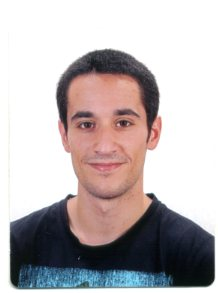
\includegraphics[width=0.6\columnwidth]{fede_fototessera.jpg}\\[\baselineskip] % Your photo
\small % Smaller font size
Federico Massa \\ % Your name
\url{fedemassa91@gmail.com}  \\
%\url{gmail.com} \\ % Your email address
%\url{www.johnsmith.com} \\ % Your URL
(+39) 347-7034248 \\ % Your phone number
\Sep % Some whitespace
\textbf{Indirizzo} \\
Via G. B. Pellizzi, 6 \\ % Address 1
56127 Pisa (PI) \\ % Address 2
Italy \\ % Address 3
\vfill % Whitespace under this block to push it up under the photo
\end{flushright}
}

%----------------------------------------------------------------------------------------

\begin{document}

\userinformation % Print your information in the left column

\framebreak % End of the first column

%----------------------------------------------------------------------------------------
%	HEADING
%----------------------------------------------------------------------------------------

\cvheading{Federico Massa} % Large heading - your name

\cvsubheading{Fisico} % Subheading - your occupation/specialization

%----------------------------------------------------------------------------------------
%	ABOUT ME
%----------------------------------------------------------------------------------------

%----------------------------------------------------------------------------------------
%	EDUCATION
%----------------------------------------------------------------------------------------

\CVSection{Istruzione}

%------------------------------------------------
\CVItem{2017 - in corso, Università di Pisa}{PhD in Ingegneria dell'Informazione presso Centro E. Piaggio}

\CVItem{2016 - 2017, Formazione post-lauream, Universit\`a di Pisa}{Corsi di Robotica (Prof. A. Bicchi), Teoria Dei Sistemi (Prof.ssa L. Pallottino), Sistemi Robotici Distribuiti (Prof.ssa L. Pallottino), Identificazione di sistemi incerti (Prof. A. Caiti) presso la Facolt\`a di Ingegneria.}

\CVItem{2013 - 2016, Universit\`a di Pisa}{Laurea Magistrale in Fisica (curriculum Interazioni Fondamentali)\\ - 110/110 e lode.\\
- Titolo della tesi: ``Tracking performances of the ATLAS detector for the\\ HL-LHC and impact on 
the H $\rightarrow 4\mu$ channel''.}

%------------------------------------------------


\CVItem{2010 - 2013, Universit\`a degli Studi di Cagliari}{Laurea Triennale in Fisica - 110/110 e lode.\\
- Titolo della tesi: ``Impact of physics beyond the Standard Model on the diffusion of neutrinos on polarized electrons''.}

%------------------------------------------------

\CVItem{2010 - 2015}{Vincitore degli Assegni di Merito della Regione Sardegna}

\CVItem{2005 - 2010, Liceo Scientifico Pitagora - Selargius (CA)}{Diploma di Maturit\`a Scientifica - 100/100 e lode.}



\CVSection{Esperienze}

\CVItem{21 - 25 Maggio 2018: Istanbul}{Scuola di Dottorato EECI "Control-oriented modeling and system identification" presso Yildiz Technical University}

\CVItem{7 - 11 Maggio 2018: Zurigo}{Scuola di Dottorato EECI "Distributed Computation and Control" presso ETH}

\CVItem{5 - 22 Marzo 2018: Banbury (UK)}{Collaborazione con azienda Roborace} 

\CVItem{8 - 15 Febbraio 2018: Firenze}{Scuola di Dottorato "Introduction to Deep Learning with Keras"}

\CVItem{Novembre 2016 - Ottobre 2017: Pisa}{Contratto di collaborazione presso il Centro Ricerche E. Piaggio}

\CVItem{Febbraio 2016: CERN (Ginevra)}{Stage al CERN per 
collaborazione con gruppo di ricerca ITk}

\CVItem{5 - 10 Giugno 2016: Alghero}{Partecipazione al workshop \textit{XIII Seminar on Nuclear, Subnuclear and Applied Physics}}

\CVItem{20 Luglio - 1 Agosto 2014: Göttingen}{Partecipazione alla \textit{HASCO Summer School on Hadron Colliders}}

\clearpage
\userinformation
\framebreak

\Sep % Extra whitespace after the end of a major section
\CVItem{Presso il Centro E. Piaggio: }{
Il mio lavoro presso il Centro E. Piaggio ha riguardato principalmente applicazioni di guida autonoma. Durante il 2017 mi sono dedicato principalmente allo studio e alla simulazione di \textbf{tecniche distribuite per il coordinamento di veicoli autonomi}. In particolare, il lavoro \`e stato incentrato sulla definizione di algoritmi di controllo per automobili che viaggiano in \textit{platooning} in un contesto autostradale. Partendo da questo ambito applicativo, \`e stato sviluppato un framework generale per la risoluzione  del problema della \textbf{intrusion detection} per sistemi multi-robot cooperanti. Lo scopo \`e stato quello di sviluppare un algoritmo distribuito che permettesse ad ogni veicolo di verificare se il comportamento osservato nei vicini fosse consistente con un certo set di regole di cooperazione.\\

Nel 2018 è stata formata presso il nostro Centro di Ricerca la prima squadra di auto autonome da corsa italiana, nell'ambito dell'evento \textbf{Roborace}, organizzato dall'azienda inglese omonima. La dinamica attuale di questo evento è quella di fornire una vettura elettrica da corsa completa di sensori, e dare alle squadre partecipanti la possibilità di progettare la propria intelligenza artificiale con lo scopo di battere il tempo di un pilota umano sfidante su un circuito di Formula E. Il mio contributo all'interno della squadra ha riguardato fondamentalmente la mappatura dell'ambiente e la localizzazione real-time del veicolo nella pista. \\

Attualmente i miei studi vertono su applicazioni innovative di \textbf{tecniche di apprendimento intelligente} (Deep Learning) e \textbf{teoria dei giochi} nei campi della robotica e della guida autonoma. }
%----------------------------------------------------------------------------------------
%	EXPERIENCE
%----------------------------------------------------------------------------------------

%\CVSection{Experience}

%------------------------------------------------

%------------------------------------------------

%------------------------------------------------


\Sep % Extra whitespace after the end of a major section

%----------------------------------------------------------------------------------------
%	COMMUNICATION SKILLS
%----------------------------------------------------------------------------------------
\CVSection{Competenze linguistiche}
\begin{table}[h!]
\centering
\resizebox{.71\textwidth}{!}{\tabulinesep=1.2mm{\begin{tabu}{| l | c | c | c | c | c |}
\cline{2-6}
\multicolumn{1}{c}{ } & \multicolumn{2}{|c|}{\textbf{Comprensione}} & \multicolumn{2}{c|}{\textbf{Orale}} & \textbf{Produzione scritta} \\ \cline{2-6}
\multicolumn{1}{c}{ } & \multicolumn{1}{|c|}{Ascolto} & Lettura & Interazione & Produzione & \\ \hline
Inglese & C1 & C1 & C1 & C1 & C1 \\ \hline
Spagnolo & B2 & B2 & B2 & B2 & B2 \\ \hline
\end{tabu}}}
\end{table}

\Sep 

\CVSection{Abilità di comunicazione}

%------------------------------------------------

Il mondo della ricerca si basa altamente sulla collaborazione e la condivisione di informazioni sia all'interno del proprio ambiente di lavoro che all'esterno. Per questo motivo è stato necessario sviluppare l'abilità di trasmettere ad altri il contenuto e il valore del proprio lavoro. In questo contesto il "pubblico" è tipicamente 
esperto, quantomeno riguardo tematiche vicine a quelle esposte. Fin dall'adolescenza, tuttavia, sono stato profondamente attratto dalla possibilità di trasmettere le mie conoscenze e soprattutto le mie passioni a persone
che fossero anche praticamente ignare di tali tematiche. Per questa ragione mi sono sempre dedicato con passione all'assistenza allo studio a ragazzi e ragazze dalle scuole medie fino a quelle superiori e oltre, 
cercando sempre di andare oltre le necessità prettamente scolastiche, sperimentando anche tecniche didattiche più interattive rispetto alla tipica lezione frontale.

%------------------------------------------------
\clearpage
\userinformation
\framebreak

%----------------------------------------------------------------------------------------
%	SKILLS
%----------------------------------------------------------------------------------------

\CVSection{Abilità specifiche}
\begin{itemize}
\item Reinforcement Learning
\item Modellizzazione e simulazione di sistemi robotici distribuiti e cooperanti;
\item Analisi matematica;
\item Meccanica classica e quantistica;
\item Elettromagnetismo;
\item Analisi statistica dei dati;
\item Fondamenti di elettronica digitale e analogica;
\item Simulazioni Monte Carlo;
\item Image processing e Computer Vision.
\end{itemize}

\Sep

\CVSection{Abilità informatiche}

%------------------------------------------------

\CVItem{Programmazione}
{\begin{tabular}{p{0.2\textwidth} p{0.2\textwidth} p{0.2\textwidth}}
\bluebullet C++ &  \bluebullet Java & \bluebullet Shell Unix\\
\bluebullet Python & \bluebullet MATLAB& \bluebullet Visual Basic \\
\bluebullet C & \bluebullet LaTeX &\\
\end{tabular}}

%------------------------------------------------

\CVItem{Sistemi operativi}
{\begin{tabular}{p{0.2\textwidth} p{0.2\textwidth} p{0.2\textwidth}}
 \bluebullet Windows &  \bluebullet Unix/Linux & \bluebullet Android\\
\end{tabular}}

%-----------------------------------------------

\CVItem{Software utilizzati}
{\begin{tabular}{p{0.2\textwidth} p{0.2\textwidth} p{0.2\textwidth}}
 \bluebullet ROOT framework & \bluebullet Geant4 framework & \bluebullet Gnuplot \\
 \bluebullet Android Studio & \bluebullet Qt Creator & \bluebullet Eclipse \\
 \bluebullet Matlab e SimuLink & \bluebullet Texmaker (editor) & \bluebullet{Unreal Engine 4} \\
\end{tabular}}

Tra i vari linguaggi, ho una lunga esperienza di programmazione in C++ (in particolare per la simulazione del rivelatore di particelle effettuata durante il periodo di tesi e per la simulazione di sistemi robotici cooperanti) e Java.\\

%------------------------------------------------

\Sep % Extra whitespace after the end of a major section

%----------------------------------------------------------------------------------------
%	NEW PAGE DELIMITER
%	Place this block wherever you would like the content of your CV to go onto the next page
%----------------------------------------------------------------------------------------

%----------------------------------------------------------------------------------------
%	AWARDS
%----------------------------------------------------------------------------------------

%\CVSection{Awards}

%------------------------------------------------

%\CVItem{2010, \textit{Postgraduate Scholarship}, Cornell University}{Awarded to the top student in their final year of a Bachelors degree.}

%------------------------------------------------

%\Sep % Extra whitespace after the end of a major section

%----------------------------------------------------------------------------------------
%	INTERESTS
%----------------------------------------------------------------------------------------

\CVSection{Interessi}

%------------------------------------------------

\CVItem{Professionali}{Sviluppo software per dispositivi mobili e desktop, Intelligenza Artificiale, Teoria dei giochi.}

%------------------------------------------------

\CVItem{Personali}{Programmazione Arduino, Musica,  
mountain-bike, video-games.}

%------------------------------------------------

\Sep % Extra whitespace after the end of a major section

%----------------------------------------------------------------------------------------
%\CVSection{Allegati}
%
%\textit{Certificato di Laurea Triennale con esami}\\
%\textit{Certificato di Laurea Magistrale con esami}\\
%\textit{Certificato di lingua inglese}\\
%\textit{Certificato di lingua spagnola}\\
%\textit{Certificato di superamento del test finale al workshop ad Alghero}\\
%\textit{Fotocopia del Documento di Identit\`a}\\
%
%\bigskip
%\textit{Autorizzo il trattamento dei miei dati personali, ai sensi del D.lgs. 196 del 30 giugno 2003.}\\

\end{document}
